\documentclass{article}
\title{\textbf{High-end Bootloaders}}
\author{}
\date{} 

\UseRawInputEncoding
\usepackage{graphicx}
\usepackage{hyperref}
\hypersetup{
    colorlinks=true,
    linkcolor=blue,
    filecolor=magenta,      
    urlcolor=cyan,
}
 
\urlstyle{same}

% Code Coloring
\usepackage{listings}
\usepackage{color}

\definecolor{dkgreen}{rgb}{0,0.6,0}
\definecolor{gray}{rgb}{0.5,0.5,0.5}
\definecolor{mauve}{rgb}{0.58,0,0.82}
\lstset{frame=tb,
  language=C++,
  aboveskip=3mm,
  belowskip=3mm,
  showstringspaces=false,
  columns=flexible,
  basicstyle={\small\ttfamily},
  numbers=none,
  numberstyle=\tiny\color{gray},
  keywordstyle=\color{blue},
  commentstyle=\color{dkgreen},
  stringstyle=\color{mauve},
  breaklines=true,
  breakatwhitespace=true,
  tabsize=3
}

%Box Note
\usepackage{graphicx}
\usepackage{tcolorbox}
\tcbuselibrary{skins}
\usepackage{lipsum}
\definecolor{boxTitle}{HTML}{fff79a}
\definecolor{boxBackground}{HTML}{fffce0}
\definecolor{boxFrame}{HTML}{f1e2b8}

\tcbset{my box/.style={
    enhanced, fonttitle=\bfseries,
    colback=boxBackground, colframe=boxFrame,
    coltitle=black, colbacktitle=boxTitle,
    attach boxed title to top left={xshift=0.3cm,
                                    yshift*=-\tcboxedtitleheight/2},
    boxed title style={
      before upper=\hspace*{0.5cm}, % reserve space for the image
      overlay={
       \node at ([xshift=0.5cm]frame.west)
         {\includegraphics[scale=0.65]{bc-dodecaedre}};
      }
    }
  }
}

\newtcolorbox{mybox}[1][]{my box, #1}


\begin{document}
\maketitle
\tableofcontents
\lstlistoflistings
\maketitle
\tableofcontents{}
\section{The Linux booting process}
In order to make the Linux kernel up and running, it will be loaded according to the following stages/process 

\begin{center}
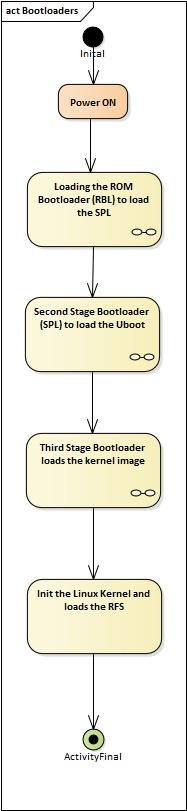
\includegraphics[scale=0.50]{./resources/img/Bootloaders.png}
\end{center}

\begin{enumerate}
    \item RBL - ROM bootloader or called the first stage bootloader\\
    This kind of bootloader resides in the ROM or flash, and It's most likely created by the SOC vendor.\\ 
    It's main purpose is to initialize the environment (e.g. Clock init, WDG timer, and the stack setup) for the second stage bootloader and then to run it.  
    \begin{itemize}
        \item It initializes the stack, clock, and the WDG timer
        \item Search in available boot interfaces for the SPL
        \item Loads the SPL (according to its image header) from the provided interface to the internal RAM memory.
        \item Executes and gives the control to the SPL.
    \end{itemize}
    
    Note: \textit{You need to visit your SoC datasheet for boot sequence, and the different boot options and interfaces (e.g. SPI booting, Ethernet Booting, eMMC, SD memory, ...)} 

    \item  SPL - Second stage bootloader or Memory bootloader\\
    It initializes the needed environment for the third stage bootloader and then run it.

    Let's say that the SPL resides in the SD card, then the RL will search on the file with a specific image header then loaded it to the internal SoC RAM.
    It's purpose
    \begin{itemize}
        \item It initializes the console to print the boot messages (e.g. UART)
        \item It initializes the external RAM memory preparing for the third stage bootloader to run
        \item Copy the third stage bootloader image according to its image header (contains start address and image size) from the boot interface to the external RAM
        \item Executes and gives the control to the third stage bootloader.
    \end{itemize}
    
    Q: \textit{Why do we need SPL ?} \\
    A: \textit{The second stage bootloader has limited size reaches few Kbytes which can't be reached by Uboot size} 

    \item Third stage bootloader, like grub or Uboot in our case it's Uboot
        It's responsible for loading the Linux image and passes the command line arguments to it.

        \begin{itemize}
            \item It initializes some peripherals like the USB or i2C or Ethernet (as configured) to load the kernel image from. (for example boot over ethernet)
            \item Loads the Linux kernel for the defined sources to the External RAM, passes the command line parameters to it and then boot. 
            Note: Booting and Configuring the uBoot at boot time can be modified by the uBoot configuration file \textbf{"uEnv.txt"} (you can override the default behaviors of uBoot by this file)
        \end{itemize} 

    \item The Linux Kernel bootstrapper, it's main function is to decompress the Linux Kernel
    \item The RFS - Root File System
\end{enumerate}


\section{Demo1 - Booting use case ``raspberry pi 1 Model B Rev 2"}
\subsection{Info about the SoC used, and the booting options}
The used HW is \href{https://raspberry-projects.com/pi/pi-hardware/raspberry-pi-model-b/model-b-io-pins}{raspberry pi 1} Model B (2011.12 Model B Revision 2.0) board with the BC

\subsection{The Pi boot Process}
\begin{enumerate}
    \item After Power ON, the GPU starts and loads the ROM bootloader which loads the 2nd stage bootloader \textbf{"bootcode.bin"} into the L2 Cache (Till now the External RAM is not initialized yet)
    \item the 2nd Stage bootloader enables the external SDRAM and loads 3rd stage bootloader \textbf{"loader.bin"} into it.
    \item 3rd Stage bootloader runs the GPU firmware \textbf{"start.elf"}, which loads the kernel image based on the configuration file \textbf{"config.txt"} which has the information of the kernel to load
    \item The 3rd stage bootloader reads \textbf{config.txt}, \textbf{cmdline.txt} and the \textbf{.dtb} (related to your board) If the dtb file exists, and then runs the \textbf{"kernel.img"} file.
    Note: In our case we will use the \textbf{config.txt} file run uBoot instead of the kernel.img file, then let the uBoot load the kernel.img.

    \begin{center}
        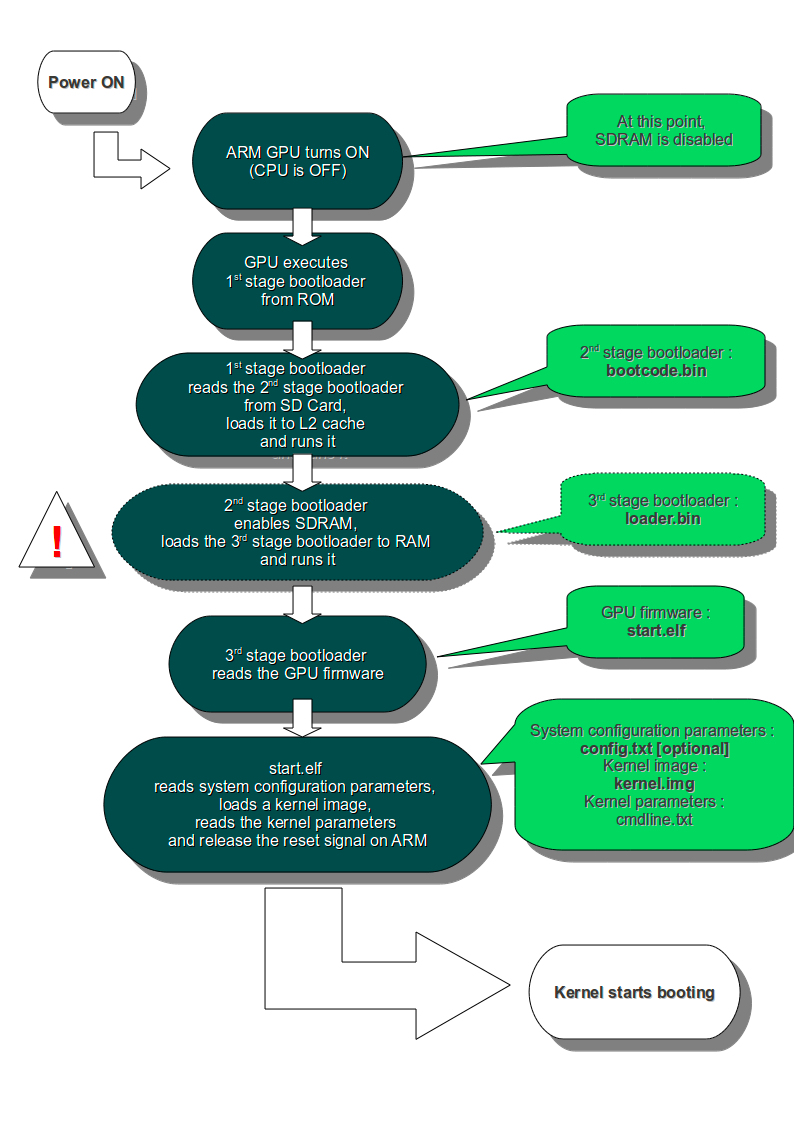
\includegraphics[scale=0.50]{./resources/img/pi-bootprocess.png}
    \end{center}
\end{enumerate}

\begin{mybox}[title={For more info about the Pi boot sequence}]
    \begin{enumerate}
        \item \href{https://www.raspberrypi.org/documentation/hardware/raspberrypi/bootmodes/bootflow.md}{The boot flow}
        \item \href{https://www.raspberrypi.org/documentation/configuration/boot_folder.md}{The contents of the boot partition}, and the prebuild images for the Pi bootloaders \href{https://github.com/raspberrypi/firmware/tree/master/boot}{here}
        \item \href{https://www.raspberrypi.org/documentation/configuration/config-txt}{The config.txt file}
    \end{enumerate}
\end{mybox}


\subsection{Building uBoot for Pi}
\subsubsection{Before we start - the prerequisites}
\begin{itemize}
    \item The needed HW
    \begin{enumerate}
        \item raspberry pi board
        \item FTDI Usb-Serial converter (and download and install the FTDI driver) to communicate to the kernel in the board
    \end{enumerate}
    \item The needed tools
    \begin{enumerate}
        \item The cross-platform compliers (will be discussed later)
        \item Uboot tools (for \textbf{mkimage} tool)
        \lstinputlisting[language=C, caption=Uboot tools installation]{./resources/src/prerequisties/installing-uboot-tools}
        \item Needed libs to install in Linux
        \lstinputlisting[language=C, caption=Config tools]{./resources/src/prerequisties/install-othertools}
        \item Install the device tree complier
        \lstinputlisting[language=C, caption=Config tools]{./resources/src/prerequisties/install-devicetreecompiler}
        \item Serial client SW like Putty or Minicom
    \end{enumerate}
\end{itemize}

The build process for uBoot is fairly simple, just three main steps;
\begin{enumerate}
    \item setup the toolchain. 
    \item configure uBoot.
    \item compile it!, that's it.
\end{enumerate}


\subsubsection{1. Setting up the Cross-Platform Complier}
In order to compile Uboot or the Linux kernel for an embedded device, we need to cross-platform toolchain, for ARM we have variety set of toolchains as follow:
\begin{itemize}
    \item Using the ARM foundation tools (baremetal tools)
    \lstinputlisting[language=C, caption=Use ARM foundation cross-compliers]{./resources/src/complie-uboot/use-arm-tools}

    \item Using Linux foundation tools
    \lstinputlisting[language=C, caption=Use Linux foundation ARM cross-compliers]{./resources/src/complie-uboot/use-linux-tools}

    \item Use Raspberrypi tools
    \lstinputlisting[language=C, caption=Use Raspberrypi tools]{./resources/src/complie-uboot/use-pi-tools}

    \item Using Linaro tools (We will be using this as it has a new version of GCC) 
    \lstinputlisting[language=C, caption=Use Linaro ARM cross-compliers]{./resources/src/complie-uboot/SetupLinaro}

    For any used toolchain, you need to export the \textbf{ARCH}, and \textbf{CROSS\_COMPILE} environmental varaibles.
    \lstinputlisting[language=C, caption=Setup the environment]{./resources/src/complie-uboot/export_cross-compile}

    Also note that every time you compile you need to set the mentioned environmental variables to the corresponding values. or you can make as follow.
    \lstinputlisting[language=C, caption=Setup the environment]{./resources/src/complie-uboot/export-cross-compile-easily}

\end{itemize}

\begin{mybox}[title={Note: compiler toolchains notations}]
while using a toolchains, you might noticed that they have a notation or you can say naming conventions, and we can try to standardize as follow:\\
\textbf{arch[-vendor][-os]-abi}:
\begin{itemize}
    \item \textbf{arch} is for architecture: arm, mips, x86, i686 ... etc.
    \item \textbf{vendor} is tool chain supplier: apple,
    \item \textbf{os} is for operating system: linux, none (bare metal)
    \item \textbf{abi} is for application binary interface convention: eabi, gnueabi, gnueabihf
\end{itemize}

Examples:\\
\textbf{arm-none-linux-gnueabi}; is he toolchain that can be installed in Debian-based systems using a package manager like apt (the package is called gcc-arm-linux-gnueabi). This toolchain targets the ARM architecture, has no vendor, creates binaries that run on the Linux operating system, and uses the GNU EABI.\\
\textbf{x86\_64-w64-mingw32}; x86\_64 architecture means AMD64, w64 is actually mingw-w64 used as a "vendor" here, mingw32 is the same as win32 API for gcc's perspective.\\
\textbf{arm-none-eabi}; This toolchain targets the ARM architecture, has no vendor, does not target an operating system (i.e. targets a "bare metal" system), and complies with the ARM eabi.\\

\end{mybox}

Finally you need to notice that they are all the same in our case.

\subsubsection{2. Configure uBoot for Pi}
First we need to fetch the uBoot source from its mainline repo.
\lstinputlisting[language=C, caption=Setup the environment]{./resources/src/complie-uboot/fetching-uBoot-Source}

The next part is to configure uBoot for a certain board, for Pi 1 we use default configurations as follow 
\lstinputlisting[language=C, caption=Setup the environment]{./resources/src/complie-uboot/configure-uBoot-for-pi}

Note: For other target you can use \textit{make help} in your uBoot root source tree, it will list all the makefile targets. or use one of the following:
\begin{itemize}
    \item rpi\_0\_defconfig -for Pi 0
    \item rpi\_defconfig - for Pi 1
    \item rpi\_2\_defconfig - for Pi 2
    \item rpi\_3\_defconfig - for Pi 3
\end{itemize}

\subsubsection{Compile uBoot}

\lstinputlisting[language=C, caption=Setup the environment]{./resources/src/complie-uboot/build!}


\subsection{U-boot environment parameters and the uEnv.txt}
The Uboot environmental variables file uEnv.txt is used to configure or override the uBoot behavior.\\
The file is straight forward key-pair (name=value) configurations (environmental variables) and embedded commands.  

\lstinputlisting[language=C, caption=Sample uEnv.txt file]{./resources/src/sample-uEnv.txt}

\begin{center}
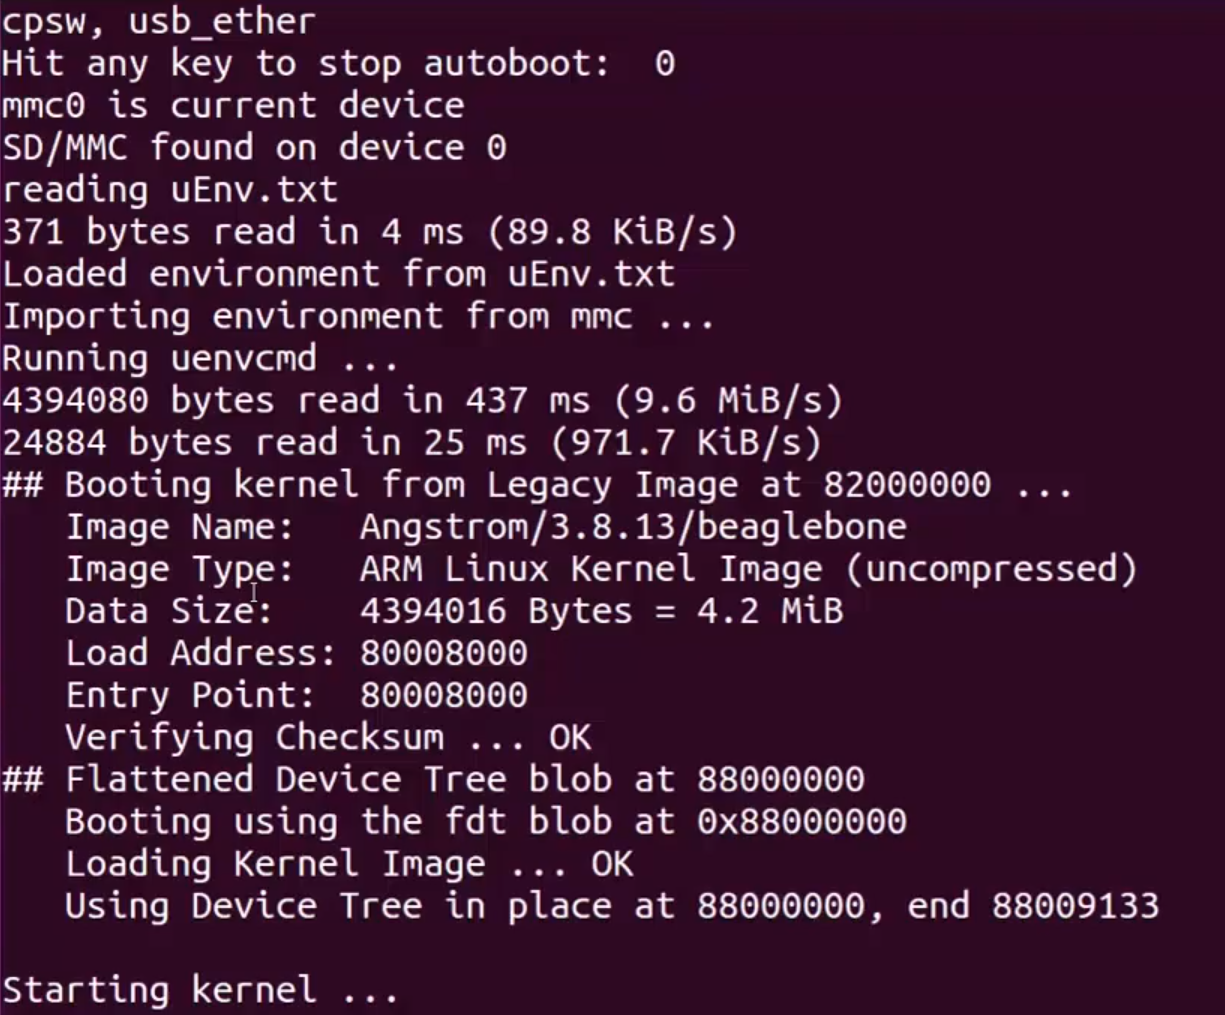
\includegraphics[scale=0.50]{./resources/img/uboot-logs01.png}
\end{center}

As you can see, the line "reading uEnv.txt", and then in order loading the kernel and the FDT into memory.


\subsection{boot.scr.uimg File}

\subsection{U-boot Kernel Image types}
The Linux kernel can be formed into different images for the uBoot to understand as following:
\begin{itemize}
    \item Linux Kernel RAW image (called uImage) and this is not used by uBoot
    \item uBoot legacy compressed image (called zImage), and it's the same as uImage but with the uBoot header create by the uBoot tool \textit{mkimage} (discussed in the example)
    
    \begin{center}
    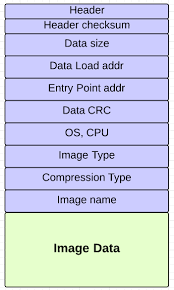
\includegraphics[scale=0.50]{./resources/img/zImage.png}
    \end{center}

    Note: the Legacy Format Image header can be found in "/include/image.h" in the uBoot source tree, and it contains:
    \lstinputlisting[language=C, caption=Legacy Format Image header struture in /include/image.h]{./resources/src/uboot_legacy_img_header}

    \item FIT Image, or the uBoot new image format which is used in Verified (secure) booting
\end{itemize}

\subsection{The Flatten Device Tree}
It's a file used to describe all the platform (board) peripherals in a static way in order for the Linux Kernel to know them. and they are board specific.\\
the details for every board is detailed in a DTS (device tree source), and then complied with a device tree complier (dtc) to form the Device Tree Binary (DTB) 

\lstinputlisting[language=C, caption=FDT syntax example]{./resources/src/fdt-syntax}

For more info about how to write a device tree, refer to The used HW is \href{https://www.raspberrypi.org/documentation/configuration/device-tree.md}{the Pi documentation}.
Note: The DTS is detailing the passive elements on the board which means something like the USB will not be listed there, as the USB device is not in the device tree as it has the ability to announce the Linux kernel its existence at runtime.

\subsection{Serial booting}
Without using SD Card, Serial booting means transferring the image to the board through the serial port (UART), so the host system will contain the bootloader, Linux image, DTB file, and RFS.\\

And you need to note that here we will use a RAM based filesystem to work with our kernel.\

\begin{mybox}[title={Note: Serial file transfer protocols}]
    In order to transfer data/files through UART, so we might be using one of the serial file transfer protocols like xModem, yModem, or zModem, kermit... .
\end{mybox}

So after booting up with the RBL, it listens on the UART using the xmodem protocol for example waiting for the first stage bootloader from the host machine, if there is a response then it will load the first stage bootloader into it's internal RAM, then the first stage bootloader will wait again through the xModem to get the second stage bootloader (e.g. uBoot), and the same for the RFS.

\subsubsection{Serial Booting using Raspberry pi using minicom}

\subsection{TFTP Booting}
Using TFTP protocol you can transfer the Linux kernel image to your board from your host. and your board will act as TFTP client with a defined IP address, and your host will be the server with a known IP address.

In order to do that we will put the \textbf{SPL, uBoot and uEnv.txt} in the SD Card, and the Linux Kernel, DTB file, and RFS in our host machine at this location /var/lib/tftpboot. \\

\section{Secure booting}

\begin{center}
    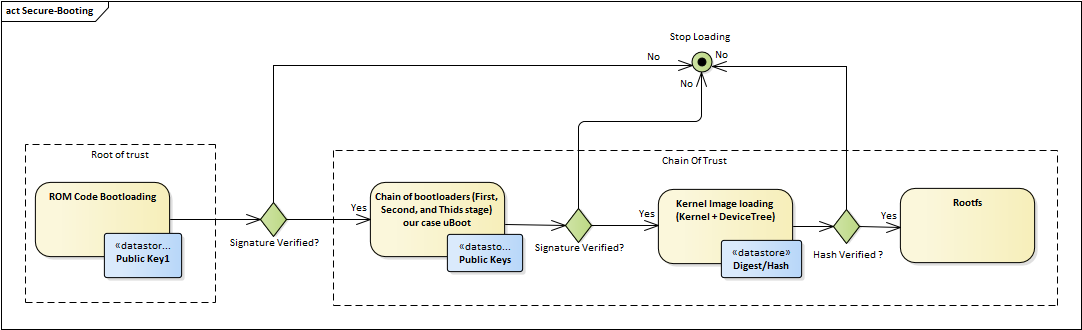
\includegraphics[scale=0.40]{./resources/img/Secure-Booting.png}
\end{center}

\subsection{Chain of trust}

The chain of trust is identified as a security verification method to verify a chain of processes from starting the CPU till we reach the applications up and running in a chained order which every node verifies that the next node will be trusty loaded. and the security is established by requiring that no code will be executed by firmware unless it has been signed by a “trusted” key.

The chain of trust uses a public key cryptography to verify the signature of the next loaded node, if the signature is invalid, then this mean that the next node is intentionally modified. 

\subsection{Root of trust}
In order to achieve a secure chain of trust, you need to make sure that the root that initialize all the secure boot process is made by a secure root/source. The root of trust is ideally based on a hardware-validated boot process to ensure the system can only be started using code from an immutable source. 

\subsection{Uboot Verified Boot - Demo on Pi}
Note: Our example with be base on RSA encryption algorithm.\\
To setup uBoot in the secure process, you need to follow the following fair and simple steps:

\begin{center}
    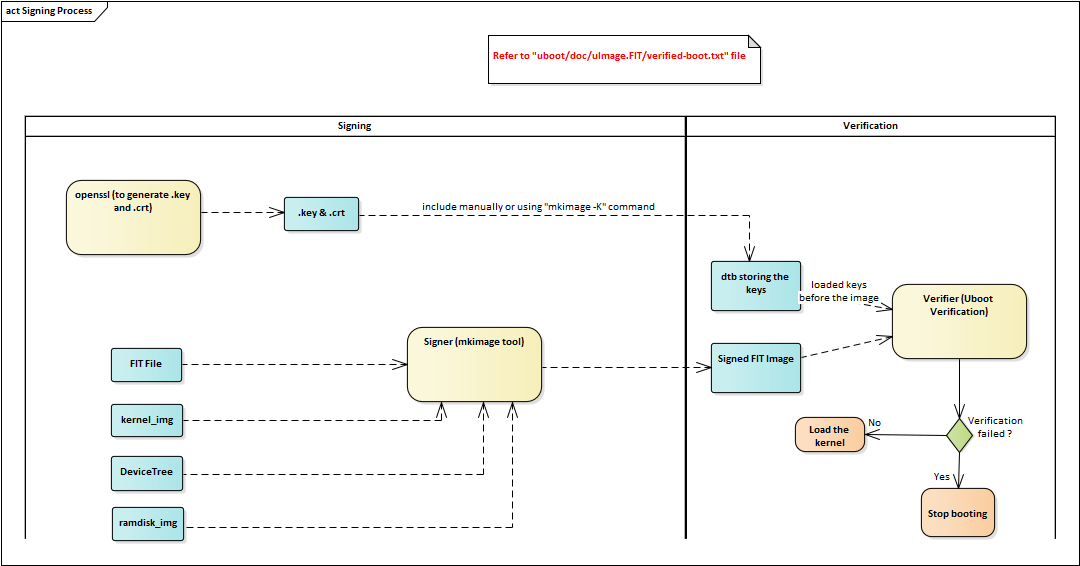
\includegraphics[scale=0.40]{./resources/img/Signing Process.png}
\end{center}

\begin{enumerate}
    \item Configuring uBoot. Before compiling uBoot. you need to configure uBoot to use FIT images and RSA algorithm. 
    The following parameters should be configured:
        \begin{itemize}
            \item Enable FIT: \textbf{CONFIG\_FIT} - enable support for the FIT uImage format
            \item Enable verified boot:
            \begin{itemize}
                \item CONFIG\_FIT\_SIGNATURE: enables signature verification of FIT images
                \item CONFIG\_RSA: enables the RSA algorithm used for FIT image verification
            \end{itemize}
        
            \item Enable FDT: CONFIG\_OF\_CONTROL, CONFIG\_OF\_SEPARATE
        \end{itemize}    
    
    \item Describe a FIT image:
        A FIT image is a extension of the old legacy image and it is tree like image that contains all files (called sub-images) required to boot a kernel, such as the kernel image, device-tree-blob and possibly a ramdisk (initrd). It follows the DeviceTree language, just create a \textbf{.its} file and follow the following example:    
        \lstinputlisting[language=C, caption=Simple FIT file]{./resources/src/verified-uboot/FIT-sample}
       
        Note: You can refer to \textbf{"doc/uImage.FIT/source\_file\_format.txt"} in the uBoot documentation folder, as a full description to create FIT formatted file.

        and you can refer to the FIT image layout as follow:
        
        \begin{center}
            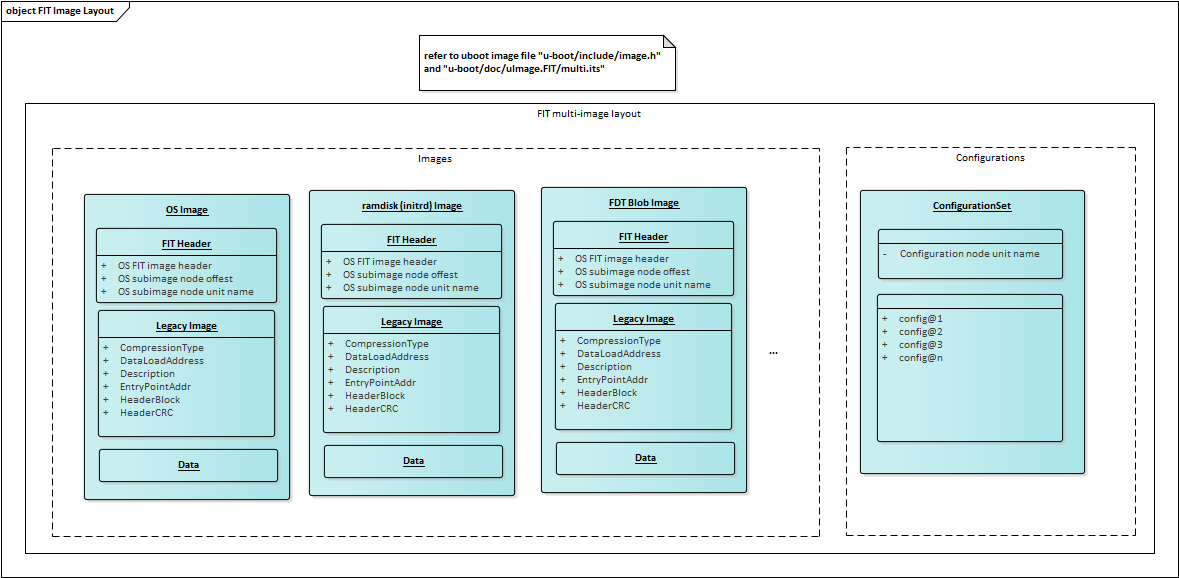
\includegraphics[scale=0.50]{./resources/img/FIT Image Layout.png}
        \end{center}

        It contains two main parts, images with a new FIT header to describe the image and its offset, and a configuration set

    \item Use the Uboot tool "mkimage" to create a FIT image from the defined FIT description file in the previous step:
    \lstinputlisting[language=C, caption=Generate a FIT image]{./resources/src/verified-uboot/generate-fit-imge}

    \item Generate the key-pair using a signer \textit{openssl}, the generated file will be a key ".key" and certificate ".crt".
    \lstinputlisting[language=C, caption=Generate Keys]{./resources/src/verified-uboot/generate-key-pair}

    \item Sign the generated FIT image. you can attach the keys by extending the FIT file as follow, and then regenerate the FIT image
    \lstinputlisting[language=C, caption=Extend the FIT file]{./resources/src/verified-uboot/sign-the-image}

    \lstinputlisting[language=C, caption=Generate the signed kernel image]{./resources/src/verified-uboot/generate-using-keys-signed-image}

    \item You can skip previous step by using the following "-f and -F" options instead, to sign the image after creating it. 
    
    The -F option is used "Indicates that an existing FIT image should be modified. No dtc compilation is performed and the -f flag should not be given. This can be used to sign images with additional keys after initial image creation." (refer to mkimage man page \href{https://manpages.debian.org/testing/u-boot-tools/mkimage.1.en.html}{here})

    \item Include the public key in uBoot device tree file
    before the verification of the image, the uBoot expects the keys to be loaded first, that's why we need to include the public key in the device tree file, and you we can achieve that by using the "-K capital k" options:
    \lstinputlisting[language=C, caption=Include the key in the dtb]{./resources/src/verified-uboot/include-publickey-in-dtb}
    
    Note: the -r option is used to tell uBoot at boot time which signature is used for certain image, otherwise uBoot will boot any signed, unsigned or wrongly signed images. if you used a signed configuration you need also to include here.
        Refer to \href{https://manpages.debian.org/testing/u-boot-tools/mkimage.1.en.html}{mkimage man page}: "Specifies that keys used to sign the FIT are required. This means that they must be verified for the image to boot. Without this option, the verification will be optional (useful for testing but not for release)."

    \item Finally try your target.
\end{enumerate}

\begin{mybox}[title={Signed Configurations to avoid mix and match attack}]
While signing images is useful, it does not provide complete protection against several types of attack. For example, it it possible to create a FIT with the same signed images, but with the configuration changed such that a different one is selected (mix and match attack). It is also possible to substitute a signed image from an older FIT version into a newer FIT (roll-back attack).\\

refer to the uBoot configuration: "uboot/doc/uImage.FIT/signature.txt"
\end{mybox}


\subsection{Playing with uboot commands}
\begin{enumerate}
    \item Load command\\\\
    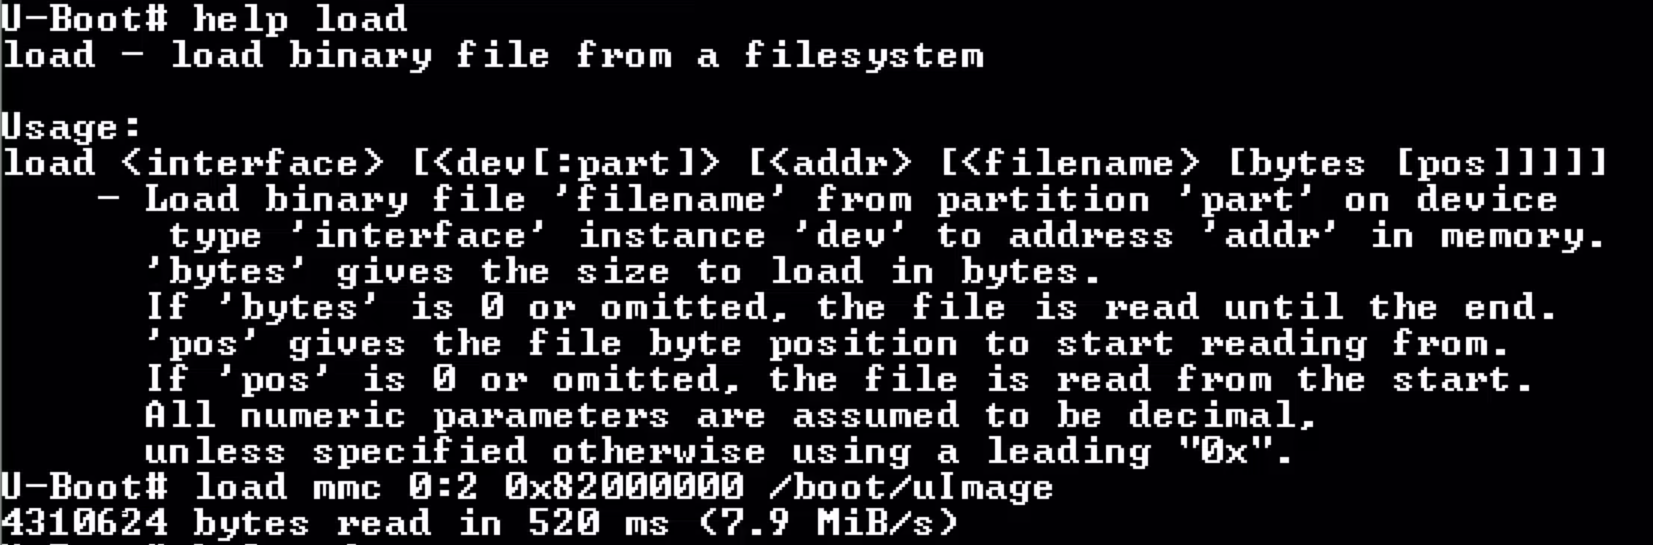
\includegraphics[scale=0.50]{./resources/img/uBootCmd-load.png}

    \item Memory Dump command\\\\
    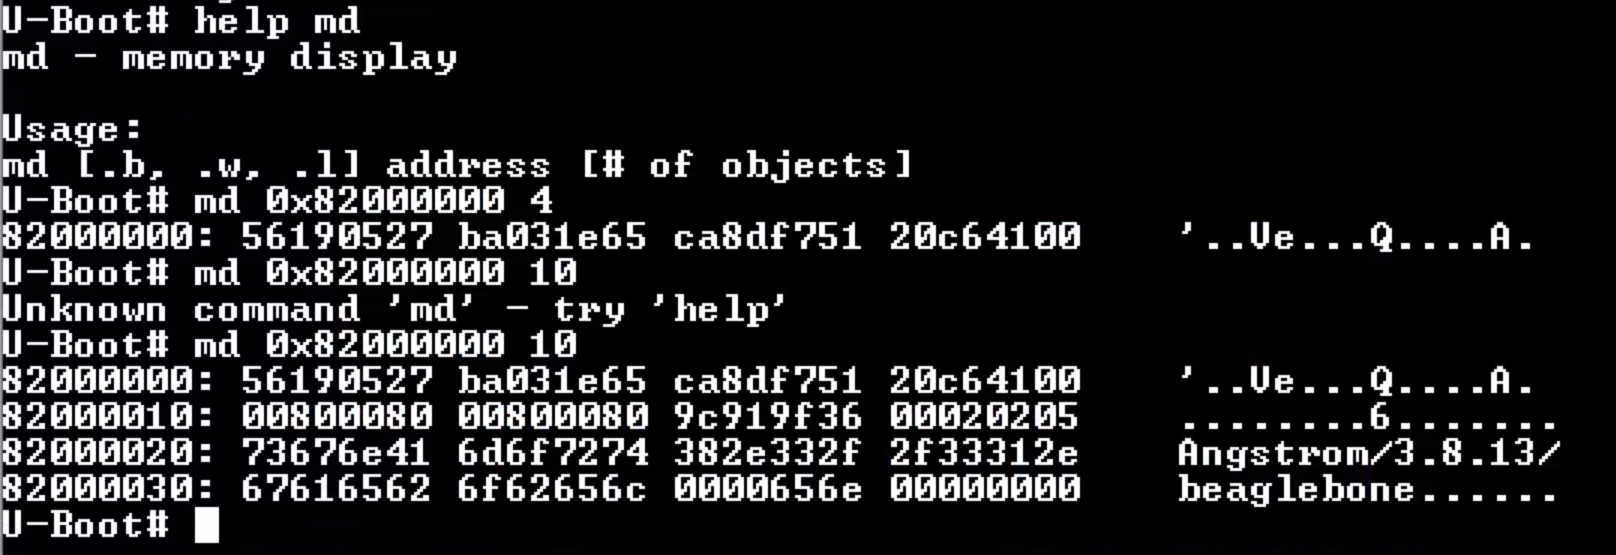
\includegraphics[scale=0.50]{./resources/img/uBootCmd-md.png}

    \item imi Comamnd\\\\
    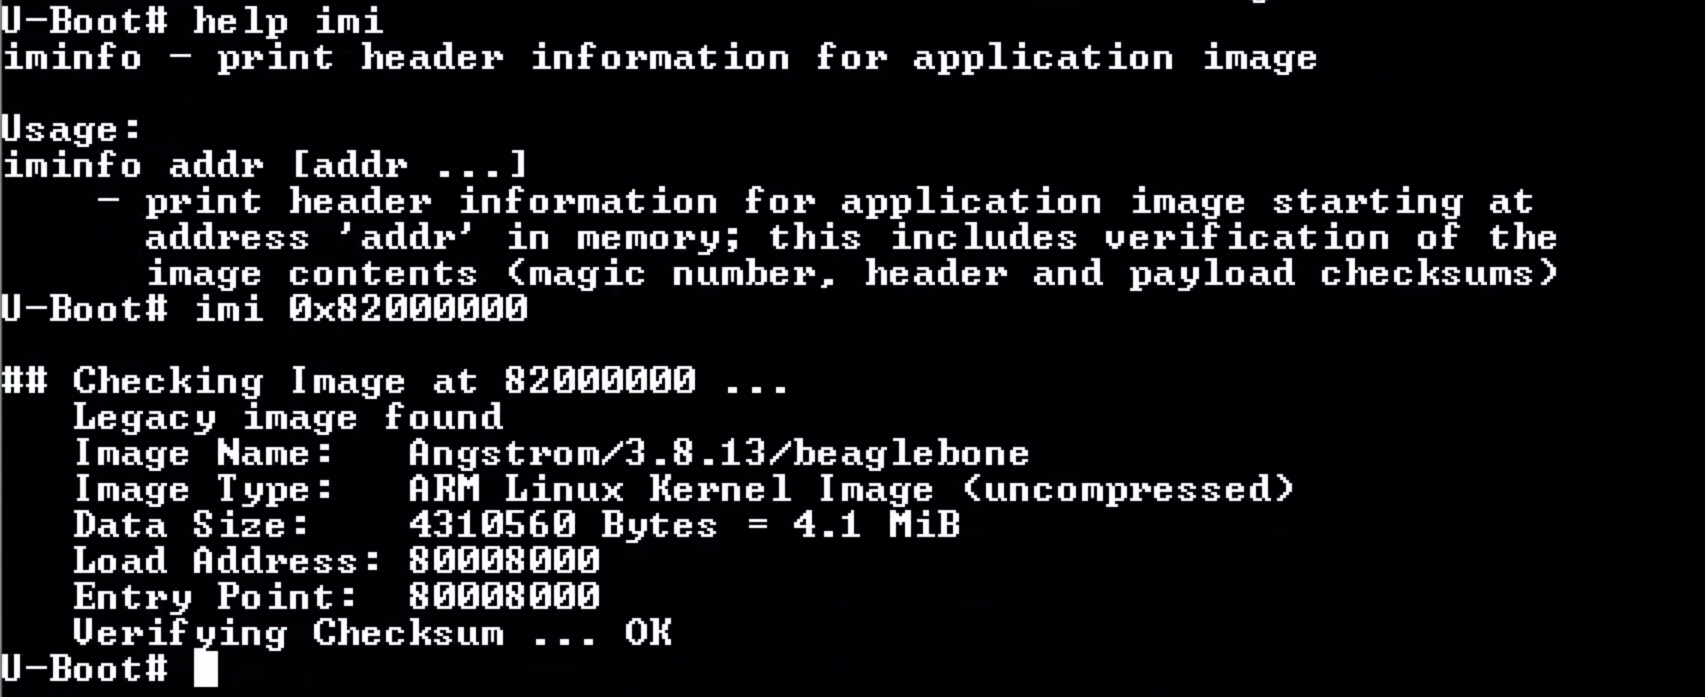
\includegraphics[scale=0.50]{./resources/img/uBootCmd-imi.png}

    \item Run command
\end{enumerate}

For the list of uBoot command visit \href{https://www.denx.de/wiki/U-Bootdoc/BasicCommandSet}{the uBoot documentation}.

\subsection{Using Uboot with BeagleBone}
\subsubsection{SoC Overview}
\subsubsection{Building for it!}
\subsection{Configuring Uboot for the PC on virtual box}

\section{References}


\end{document}